\section{METODOLOGI PENGEMBANGAN}

\subsection{Metodologi yang Dipilih}

Savora dikembangkan menggunakan pendekatan \textbf{Agile/Scrum sederhana} dengan iterasi
\textit{sprint} pendek. Metodologi ini dipilih karena durasi lomba yang terbatas menuntut tim
melakukan iterasi cepat, membagi pekerjaan ke dalam \textit{sprint}, melakukan evaluasi harian,
dan memprioritaskan fitur MVP agar produk selaras dengan kebutuhan pengguna dan RuleBook lomba.

\subsection{Alasan Pemilihan Scrum}

\begin{enumerate}[leftmargin=*]
    \item \textbf{Iterasi Cepat} : Memungkinkan pengembangan dan pengujian fitur secara bertahap, sehingga bug dapat teridentifikasi lebih awal.
    \item \textbf{Feedback Berkala} : Stakeholder dapat memberikan masukan setiap akhir sprint untuk perbaikan berkelanjutan.
    \item \textbf{Transparansi} : Daily standup dan sprint review memastikan seluruh tim memiliki pemahaman yang sama tentang progres.
    \item \textbf{Adaptif} : Perubahan prioritas atau kebutuhan dapat diakomodasi tanpa mengganggu seluruh roadmap.
\end{enumerate}

\subsection{Tahapan dan Timeline Pengembangan}

Pengembangan Savora dijalankan dalam lima tahapan utama yang dipetakan ke dalam timeline lomba
selama 22 hari (4--25 Juli 2026).

\begin{table}[htbp]
\centering
\caption{Tahapan Pengembangan Savora}
\label{tab:tahapan}
\begin{tabularx}{\textwidth}{|l|X|X|}
\hline
\textbf{Tahap} & \textbf{Fokus} & \textbf{Output} \\
\hline
Discovery \& Scope Lock & Menentukan masalah, fitur, \textit{user flow}, dan batasan MVP & PRD final dan \textit{backlog} \\
\hline
Design Sprint & Wireframe, \textit{design system}, dan prototipe & Figma dan \textit{design spec} \\
\hline
Development Sprint & Implementasi \textit{frontend}, \textit{backend}, database, dan integrasi API & MVP berjalan \textit{end-to-end} \\
\hline
Testing \& Refinement & Pengujian, \textit{bug fixing}, dan perbaikan UX & Demo stabil \\
\hline
Submission Preparation & Proposal, video demo, deployment, dan README & Paket \textit{submission} lengkap \\
\hline
\end{tabularx}
\end{table}

\begin{table}[htbp]
\centering
\caption{Timeline 22 Hari Pengembangan Savora}
\label{tab:timeline}
\begin{tabularx}{\textwidth}{|l|l|X|}
\hline
\textbf{Minggu} & \textbf{Tanggal} & \textbf{Fokus dan Deliverable} \\
\hline
W1 & 4--10 Jul & Setup repo, database, \textit{auth}, API \textit{skeleton}, dan \textit{design system} \\
\hline
W2 & 11--17 Jul & Fitur inti: marketplace, Food Trust Index, pembayaran Midtrans, Help Center, Waste Log \\
\hline
W3 & 18--22 Jul & Dashboard, rating, analitik, \textit{testing}, deploy, dan video demo \\
\hline
Deadline & 25 Jul & \textit{Submission}: proposal PDF, video, GitHub, dan aplikasi \textit{deployed} \\
\hline
\end{tabularx}
\end{table}

\begin{figure}[htbp]
\centering
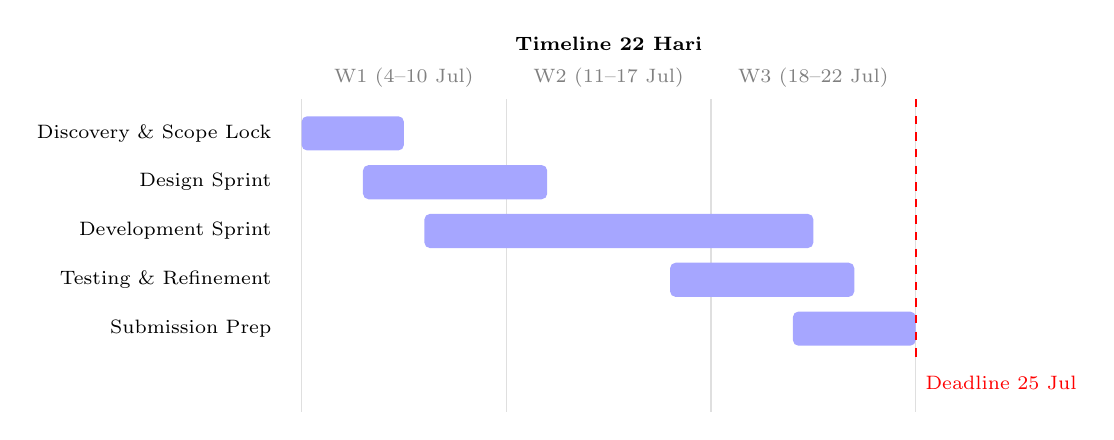
\begin{tikzpicture}[font=\scriptsize, x=2.6cm, y=0.62cm]
    % Grid minggu (3 kolom = W1, W2, W3)
    \foreach \w in {0,1,2,3} {
        \draw[gray!25] (\w,0.2) -- (\w,-6.2);
    }
    % Label minggu
    \foreach \w/\lbl in {0/{W1 (4--10 Jul)}, 1/{W2 (11--17 Jul)}, 2/{W3 (18--22 Jul)}} {
        \node[above, gray] at (\w+0.5, 0.25) {\lbl};
    }
    \node[above] at (1.5, 1.0) {\textbf{Timeline 22 Hari}};
    % Bar tahap: {row}{start}{len}{label}
    \foreach \row/\start/\len/\lbl in {
        0/0/0.5/{Discovery \& Scope Lock},
        1/0.3/0.9/{Design Sprint},
        2/0.6/1.9/{Development Sprint},
        3/1.8/0.9/{Testing \& Refinement},
        4/2.4/0.6/{Submission Prep}
    } {
        \fill[blue!35, rounded corners=2pt] (\start, -\row-0.15) rectangle (\start+\len, -\row-0.85);
        \node[left, black] at (-0.1, -\row-0.5) {\lbl};
    }
    % Milestone deadline
    \draw[red, thick, dashed] (3,0.2) -- (3,-5.2);
    \node[right, red, font=\scriptsize] at (3, -5.6) {Deadline 25 Jul};
\end{tikzpicture}
\caption{Timeline (Gantt Chart) Pengembangan Savora}
\label{fig:gantt}
\end{figure}

\subsection{Peran Anggota Tim}

\begin{table}[htbp]
\centering
\caption{Pembagian Tugas Anggota Tim}
\label{tab:peran}
\begin{tabularx}{\textwidth}{|l|Y|Y|}
\hline
\textbf{Anggota} & \textbf{Role} & \textbf{Tanggung Jawab} \\
\hline
Wa Ode Nur Alia & Auth, Admin, Keuangan, Mitra Donasi, Iklan & \textit{Auth} \& \textit{role} user, dashboard admin, keuangan platform, verifikasi mitra donasi, manajemen iklan, \textit{export} laporan \\
\hline
Richard Firmansyah & Marketplace Customer, Detail Produk, Slot Iklan & Beranda Food Score/Rescue Time, badge keyword safety, slot iklan marketplace, detail produk \\
\hline
Muhammad Rifaidi & Dashboard UMKM, Analitik, Insight, Iklan UMKM & Dashboard UMKM, analitik penjualan, \textit{insight} rating \& keyword, analitik pelacakan, pengiklanan produk \\
\hline
Ridwan Hakim Ramadhan & Food Score Decay, Keyword Classification & Rumus Food Score \textit{decay}, mesin klasifikasi keyword ulasan, API \textit{score} \& keyword \\
\hline
Nadi Azzada Akbar & Cashless, Service Fee, Order, Review Keyword & Sistem \textit{cashless} Midtrans, \textit{service fee} 5\%, checkout, \textit{order tracking}, input review keyword \\
\hline
\end{tabularx}
\end{table}

\subsection{Tools Pendukung}

\begin{itemize}[leftmargin=*]
    \item \textbf{Project Management} : Notion atau Trello untuk sprint board dan task tracking
    \item \textbf{Communication} : Discord atau WhatsApp Group untuk komunikasi harian
    \item \textbf{Design} : Figma untuk wireframe dan UI design
    \item \textbf{Documentation} : Google Docs untuk dokumentasi teknis
    \item \textbf{Version Control} : Git dengan branch strategy (main, develop, feature branches)
\end{itemize}
